\portada

\begin{esquemaExplorador}
  \temaEsquema{Correspondencia cuántica}{
    \conceptoEsquema{Amplitud cuántica}{$\alpha\in\C$}
    \conceptoEsquema{Magnitud y probabilidad}{$P = |\alpha|^2$}
    \conceptoEsquema{Fase e interferencia}{$\theta = arg(\alpha)$}
  }
  \temaEsquema{Notación bra-ket}{
    \conceptoEsquema{Kets y bras}{$\ket{a}$ y $\bra{a}$}
    \conceptoEsquema{Productos internos}{$\braket{a}{b}$}
    \conceptoEsquema{Operadores externos}{$\ketbra{a}{b}$}
  }
  \temaEsquema{Estados cuánticos}{
    \conceptoEsquema{cúbits y normalización}{}
    \conceptoEsquema{Superposición cuántica}{$\alpha\ket{0} + \beta\ket{1}$}
    \conceptoEsquema{Interpretación probabilística}{}
  }
  \temaEsquema{Sistemas de múltiples cúbits}{
    \conceptoEsquema{Producto tensorial}{$\ket{ab}$}
    \conceptoEsquema{Base computacional}{$\ket{0}, \ket{1}$}
    \conceptoEsquema{Estados entrelazados}{$\frac{1}{\sqrt{2}}\ket{00} + \ket{11}$}
  }
  \temaEsquema{Mediciones y observables}{
    \conceptoEsquema{Colapso del estado}{}
    \conceptoEsquema{Medidas en diferentes bases}{}
  }
  \temaEsquema{Dinámicas cuánticas}{
    \conceptoEsquema{Acción de operadores}{}
    \conceptoEsquema{Evolución libre}{}
  }
\end{esquemaExplorador}

\unirsection{Ideas clave}

\subsection{Introducción y objetivos}

Hasta ahora hemos explorado la columna vertebral matemática de la mecánica cuántica: los espacios vectoriales complejos y los espacios de Hilbert, en ambos casos de dimensión finita. Estos conceptos son esenciales para describir sistemas cuánticos, y en particular, los cúbits, que son la unidad fundamental de información en computación cuántica.

Ahora comienza la parte más emocionante del curso: aplicar esta base matemática para entender cómo se representan y manipulan los estados cuánticos, y cómo evolucionan y miden estos estados en los sistemas desarrollados para la computación cuántica.

Revisaremos los postulados de la mecánica cuántica, enfocándonos en su interpretación física y su formulación matemática utilizando la notación de Dirac. Esta notación es una herramienta poderosa que simplifica la representación y manipulación de estados y operadores cuánticos.

La notación de Dirac, también conocida como notación bra-ket, proporciona un formalismo elegante y poderoso para trabajar con estados cuánticos y operadores. Desarrollada por Paul Dirac, esta notación no solo simplifica los cálculos algebraicos, sino que también captura de manera intuitiva los conceptos físicos fundamentales de la mecánica cuántica.

En computación cuántica, la notación de Dirac es indispensable porque:

\begin{itemize}
  \item Proporciona una representación \textbf{concisa y clara} de estados cuánticos complejos.
  \item Facilita el cálculo de \textbf{probabilidades cuánticas} mediante productos internos.
  \item Permite expresar \textbf{operadores cuánticos} de manera natural y eficiente.
  \item Conecta directamente la \textbf{estructura matemática} con la \textbf{interpretación física}.
  \item Es el lenguaje estándar para describir \textbf{algoritmos cuánticos} y \textbf{protocolos cuánticos}.
\end{itemize}

Este tema establece el puente definitivo entre la matemática abstracta de los espacios de Hilbert y la implementación práctica de sistemas cuánticos en computación cuántica.

\begin{nota}
  Recuerda que en todo el curso, siempre trabajaremos con espacios de Hilbert de dimensión finita, lo que simplifica muchos aspectos técnicos y nos permite centrarnos en los conceptos fundamentales.
\end{nota}

En el contexto de la mecánica cuántica, un número complejo se describe como una amplitud cuántica que está formado por un par de números llamados amplitud y fase, que no son más que el módulo y un argumento.

\begin{defi}
  Se denota por \textbf{amplitud cuántica} a un número complejo $\alpha \in \C$ que está caracterizado por dos valores:
  \begin{itemize}
    \item \textbf{Magnitud}: Igual al módulo $|\alpha|$.
    \item \textbf{Fase}: Pertenece al argumento $\arg(\alpha)$.
  \end{itemize}
\end{defi}

Por lo tanto, dos amplitudes cuánticas son iguales si tienen la misma magnitud y su diferencia de fases es un múltiplo de $2\pi$.

\begin{eje}
  Una amplitud cuántica de magnitud 2 con fase $\pi$ es igual a otra amplitud cuántica de magnitud 2 con fase $-\pi$.
\end{eje}

\begin{eje}[Interferencia cuántica]
  Cuando dos amplitudes cuánticas interfieren, la amplitud cuántica resultante puede tener una fase menor, diremos entonces que las amplitudes interfieren de forma destructiva, si la fase resultante es mayor diremos que interfieren de forma constructiva:

  \textbf{Interferencia destructiva}: Una amplitud cuántica de magnitud 2 con fase $\pi$ y otra amplitud cuántica de magnitud 2 con fase $\pi$ interfieren dando una amplitud cuántica de fase $0$.

\end{eje}

\begin{info}
  La interferencia cuántica es el principio fundamental detrás de muchos algoritmos cuánticos: amplificamos las amplitudes de respuestas correctas e interferimos destructivamente con las incorrectas.
\end{info}

Al final una amplitud cuántica es la representación exponencial de un número complejo, y podemos trabajar con ellas usando las reglas vistas en este curso.

\subsection{Postulado I: Sistemas cuánticos.}
\begin{resaltado}
  Un sistema cuántico se describe completamente mediante un vector unitario en un espacio vectorial de Hilbert.
\end{resaltado}

Aunque para nosotros los espacios vectoriales y los espacios de Hilbert sean lo mismo, es a partir de ahora, cuando empezamos a diferenciar ambos conceptos. Un espacio de Hilbert es un espacio vectorial complejo con un producto interno definido, y en el contexto de la mecánica cuántica, este espacio es el \textbf{espacio de estados normalizados} del sistema cuántico.

\begin{defi}
  A los elementos de un espacio de estados $\H$, no los llamaremos vectores sino \textbf{estados cuánticos} o en la notación de Dirac \textbf{kets} y se denota por $\ket{v}\in\H$.
\end{defi}

Siempre que hablamos de estado cuántico o de ket, estamos asumiendo ya que el vector es unitario, es decir, que cumple $\|\ket{v}\| = 1$.

En computación cuántica, el sistema cuántico más básico es el \textbf{cúbit}, en el que podemos medir dos estados bien diferenciados, y por tanto es un espacio de estados $\mathcal{C}$ de dimensión 2.

Que un sistema cuántico se describa mediante un vector unitario implica que los estados cuánticos deben cumplir la \textbf{condición de normalización}, y por tanto, no todos los vectores del espacio vectorial son estados físicos válidos. Tenemos que considerar el espacio de Hilbert $\H$ como el subespacio de todos los vectores unitarios del espacio vectorial complejo asociado.

En mecánica cuántica, un ket cuando es representado por coordenadas se escribe como una columna matricial, siguiendo la convención de que las coordenadas son los coeficientes de la combinación lineal de los vectores de una base ortonormal.

\begin{eje}[Espacio de estado de un cúbit]
  Como hemos definido, un cúbit tiene espacio de estados $\mathcal{C}$ de dimensión 2 y si $\mathcal{B} = \{e_1, e_2\}$ es una base, todo estado cuántico $\ket{v}$ viene representado por
  $$\ket{v} = \alpha\ket{e_1} + \beta\ket{e_2}\quad \alpha, \beta \in \mathbb{C}\mid |\alpha|^2 + |\beta|^2 = 1\,.$$

  En computación cuántica, es habitual denotar por $\ket{0}$ y $\ket{1}$ a los estados que caracterizan el cúbit. Si por ejemplo estamos usando el spin de un electrón, estos estados pueden representar el spin \textit{arriba} y \textit{abajo} respectivamente.

  Llamaremos \textbf{base computacional} de $\mathcal{C}$ a la base $\{\ket{0}, \ket{1}\}$.
\end{eje}

Para definir formalmente $\mathcal{C}$, necesitamos imponer la condición de normalización en los vectores del espacio vectorial complejo asociado $\mathbb{C}^2$. Esto nos lleva a la siguiente construcción.

\begin{prop}
  La relación $R$ sobre $\mathbb{C}^2$ definida por
  $$v R w \iff \exists r \in \mathbb{R}\mid w = rv\,,$$
  es una relación de equivalencia.
\end{prop}
\begin{proof}
  Veamos que $R$ cumple las tres propiedades de una relación de equivalencia:
  \begin{itemize}
    \item \textbf{Reflexiva}: Para todo $v \in \mathbb{C}^2$, existe $r = 1 \in \mathbb{R}$ tal que $v = 1 \cdot v$, por lo que $v R v$.
    \item \textbf{Simétrica}: Si $v R w$, entonces existe $r \in \mathbb{R}$ tal que $w = rv$. Entonces, si $r \neq 0$, podemos escribir $v = r^{-1}w$, con $r^{-1} \in \mathbb{R}$, por lo que $w R v$. Si $r = 0$, entonces $w = 0$ y también $v = 0$, por lo que $w R v$.
    \item \textbf{Transitiva}: Si $v R w$ y $w R u$, entonces existen $r_1, r_2 \in \mathbb{R}$ tales que $w = r_1 v$ y $u = r_2 w$. Sustituyendo, obtenemos $u = r_2 (r_1 v) = (r_2 r_1) v$, con $r_2 r_1 \in \mathbb{R}$, por lo que $v R u$.
  \end{itemize}
\end{proof}

Ahora podemos establecer la relación entre los espacios formalmente, considerando $\mathcal{C}$ como el conjunto cociente $\mathbb{C}^2 / R$, y cada clase de equivalencia representa un estado cuántico físico, tomando como representante de la clase $\ket{v}$ aquel que tiene norma 1.

\begin{eje}
  Consideremos el cúbit resultado de medir el spin de un electrón en un dirección del espacio. Llamemos $\ket{\uparrow}$ al estado en el que el spin mide en dicha dirección y $\ket{\downarrow}$ al estado en el que el spin mide en la dirección opuesta.

  En este caso, $\ket{\uparrow}$ y $\ket{\downarrow}$ son los estados que forman la base computacional de $\mathcal{C}$ y podemos expresar conceptos como un estado diagonal como
  \[
    \ket{\nearrow } = \frac{1}{\sqrt{2}}(\ket{\uparrow} + \ket{\downarrow})\,.
  \]
\end{eje}

\begin{defi}[Equivalencia por fase global]
  Dos cúbits se dicen que son iguales salvo por una \textbf{fase global} si están en la misma clase de equivalencia.

  Si no están en la misma clase de equivalencia, se dicen que tienen \textbf{fases relativas}.
\end{defi}

\begin{eje}[Parametrización general de un cúbit]
  Eliminando la fase global, todo cúbit puede escribirse como
  $$\ket{v} = \cos\frac{\theta}{2}\ket{0} + e^{i\varphi}\sin\frac{\theta}{2}\ket{1}\,,$$
  donde $\theta \in [0,\pi]$ y $\varphi \in [0,2\pi)$ son parámetros reales.

  Esta parametrización:
  \begin{itemize}
    \item Elimina la fase global irrelevante.
    \item Usa solo 2 parámetros reales para describir el estado completo.
    \item Corresponde a puntos en la superficie de una esfera (Esfera de Bloch).
  \end{itemize}
\end{eje}

En computación cuántica, una vez definido los estados básicos que forman la base computacional, tenemos otros estados importantes que usaremos a lo largo del curso.
\begin{enumerate}
  \item $\ket{+} = \frac{1}{\sqrt{2}}(\ket{0} + \ket{1})$.
  \item $\ket{-} = \frac{1}{\sqrt{2}}(\ket{0} - \ket{1})$.
  \item $\ket{i+} = \frac{1}{\sqrt{2}}(\ket{0} + i\ket{1})$.
  \item $\ket{i-} = \frac{1}{\sqrt{2}}(\ket{0} - i\ket{1})$.
\end{enumerate}

\begin{defi}[Bracket]
  En la notación de Dirac, el \textbf{bracket} es el producto interno entre dos kets $\ket{v}$ y $\ket{w}$, se denota $\braket{v}{w}$
  $$\braket{v}{w} = \langle v , w \rangle \in \C\,.$$
\end{defi}

Recordando la definición del dual de un espacio vectorial, dado un ket $\ket{v}$, el funcional asociado es un elemento del espacio dual $\H^*$, que podría verse como un producto interno para cierto $\ket{w}$ y que con la notación de Dirac tiene sentido dar la siguiente definición.

\begin{defi}[Bra]
  Dado un ket $\ket{\phi}$, el funcional asociado del espacio dual lo llamamos \textbf{bra}, denotado $\bra{\phi}$ y que actúa sobre un ket $\ket{v}$ mediante la notación
  $$\bra{\phi}(\ket{v}) = \braket{\phi}{v}\,.$$
\end{defi}

Para cada ket $\ket{v}$, el bra correspondiente respecto de una base ortogonal y su base dual cumple
$$\bra{v} = \ket{v}^\dagger\,.$$

\subsection{Postulado II: Observables}

\begin{resaltado}
  Toda magnitud física observable de un sistema cuántico se representa mediante un operador hermitiano que actúa en el espacio de Hilbert del sistema y cuyos valores propios son todos los posibles valores que podemos observar.
\end{resaltado}

Este postulado nos indica, que dado un cúbit, y fijado los estados básicos que lo definen, tendremos operadores hermíticos que actúan sobre el cúbit y cuyos valores propios son los posibles resultados de medir la magnitud observable.

En la notación de Dirac, no se diferencia entre operadores lineales y sus representaciones matriciales, por lo que la representación matricial de un operador hermítico $T:\H\to\H$ se denota simplemente por $T$.

Tampoco se diferencia entre la imagen de un ket $\ket{v}$ por el operador $T$ o el producto de su representación matricial por la representación del vector, lo que $T\ket{v}$ significa a la misma vez la imagen del ket por el operador o el produto de la matriz por el vector columna.

\begin{eje}[Observables fundamentales de un cúbit basado en el spin]
  Para un cúbit que representa el spin de un electrón, los observables más importantes son las componentes del espín en cada una de las direcciones del espacio, representadas por las matrices de Pauli.

  \begin{align*}
    X & = \begin{pmatrix} 0 & 1 \\ 1 & 0 \end{pmatrix}  & \text{(espín en dirección x)} \\
    Y & = \begin{pmatrix} 0 & -i \\ i & 0 \end{pmatrix} & \text{(espín en dirección y)} \\
    Z & = \begin{pmatrix} 1 & 0 \\ 0 & -1 \end{pmatrix} & \text{(espín en dirección z)}
  \end{align*}
\end{eje}

La matriz de Pauli $Z$ ya es diagonal y en el tema anteriorio~\ref{eje:exponencial_x} se calculó la representación espectral de la matriz de Pauli $X$.
Veamos ahora cómo diagonalizar la matriz de Pauli $Y$, lo que nos permitirá conocer sus valores propios y vectores propios, fundamentales para entender las posibles mediciones en un sistema cuántico.

\begin{eje}[Diagonalización de $Y$]
  Para calcular los valores propios del observable $Y$, resolvemos $\det(Y - \lambda I) = 0$,
  $$\det\begin{pmatrix} -\lambda & -i \\ i & -\lambda \end{pmatrix} = \lambda^2 - 1 = 0\,.$$
  Valores propios: $\lambda_1 = 1$, $\lambda_2 = -1$.

  \textbf{Vectores propios:}
  \begin{itemize}
    \item Para $\lambda_1 = 1$: Resolvemos $(Y - I)\ket{v} = 0$
          $$\begin{pmatrix} -1 & -i \\ i & -1 \end{pmatrix}\begin{pmatrix} v_1 \\ v_2 \end{pmatrix} = 0\,.$$
          De la primera fila: $-v_1 - i v_2 = 0 \implies v_1 = -i v_2$.
          Tomando $v_2 = 1$, obtenemos $\ket{v} = (-i, 1)^t$.
    \item Para $\lambda_2 = -1$: Resolvemos $(Y + I)\ket{w} = 0$
          $$\begin{pmatrix} 1 & -i \\ i & 1 \end{pmatrix}\begin{pmatrix} w_1 \\ w_2 \end{pmatrix} = 0\,.$$
          De la primera fila: $w_1 - i w_2 = 0 \implies w_1 = i w_2$.
          Tomando $w_2 = 1$, obtenemos $\ket{w} = (i, 1)^t$.
  \end{itemize}

  \textbf{Descomposición espectral:}
  $$Y = \frac{1}{2}\begin{pmatrix}
      i & -i \\
      1 & 1
    \end{pmatrix}\begin{pmatrix}
      1 & 0  \\
      0 & -1
    \end{pmatrix}\begin{pmatrix}
      -i & 1 \\
      i  & 1
    \end{pmatrix}\,.$$
\end{eje}

\subsection{Postulado III: Medición cuántica}

\begin{resaltado}
  Al medir con un observable $T$ el estado $\ket{v}$:
  \begin{enumerate}
    \item La probabilidad de obtener el resultado $\lambda_i$ es
          $$P(\lambda_i) = \|\text{proy}_{V_i}\ket{v}\|^2\,.$$
    \item Después de la medición, el sistema se representa con el estado
          $$\ket{w} = \frac{\text{proy}_{V_i}\ket{v}}{\|\text{proy}_{V_i}\ket{v}\|}\,.$$
  \end{enumerate}
  Donde $V_i$ es el subespacio propio correspondiente al valor propio $\lambda_i$.
\end{resaltado}

El tercer postulado es menos intuitivo de todos los postulados, pues nos asegura que no sabemos que ocurre al medir, solo podemos tener un conocimiento probabilístico sobre los distintos resultados que podemos obtener.

Aunque sí podemos obtener un valor sobre dicha probabilidad, y es el módulo de la proyección del estado sobre los vectores de la base formada por los vectores propios del observable.

Si recordamos las ecuaciones del tema anterior, cuando tenemos valores propios distintos, el módulo de la proyección es precisamente el módulo del producto interno. Y por otro lado, es precisamente este valor del producto interno la coordendada del estado con respecto a la base propia.
\begin{align*}
  \ket{v}                      & = \sum_{i=1}^n \braket{e_i}{v}\ket{e_i}\,. \\
  \|\text{proy}_{e_i}\ket{v}\| & = \|\braket{e_i}{v}\|\,.
\end{align*}

\begin{eje}
  Considere el estado $\ket{v} = \frac{3}{5}\ket{0} + \frac{4i}{5}\ket{1}$ y queremos medir con el observable $Z$. Como ya sabemos, los valores propios de $Z$ son $+1$ y $-1$, con vectores propios $\ket{0}$ y $\ket{1}$ respectivamente.

  \textbf{Probabilidades:}
  \begin{align*}
    P(+1) & = |\braket{0}{v}|^2 = \left|\frac{3}{5}\right|^2 = \frac{9}{25}\,.   \\
    P(-1) & = |\braket{1}{v}|^2 = \left|\frac{4i}{5}\right|^2 = \frac{16}{25}\,.
  \end{align*}

  \textbf{Estados post-medición:} Después de cada posible resultado de la medición, el estado del sistema se representa con el estado:
  \begin{itemize}
    \item $\ket{0}$ si se obtiene $+1$.
    \item $\ket{1}$ si se obtiene $-1$.
  \end{itemize}
\end{eje}

\begin{defi}[Valor esperado]
  \label{defi:valor_esperado}
  El \textbf{valor esperado} de un observable $T$ sobre el estado $\ket{v}$ es
  $$\langle T \rangle_v = \sum_i \lambda_i P(\lambda_i)\,.$$
\end{defi}

\begin{eje}
  Para el estado $\ket{v} = \frac{3}{5}\ket{0} + \frac{4i}{5}\ket{1}$ y el observable $Z$, su valor esperado es

  $$\langle  Z \rangle_v = (+1) \cdot \frac{9}{25} + (-1) \cdot \frac{16}{25} = -\frac{7}{25}\,.$$
\end{eje}

La definición de valor esperado es una generalización del valor esperado en estadística, donde el valor esperado es la media de una variable aleatoria. Pero si realizamos algunos cálculos, podemos ver que el valor esperado es el producto interno entre el ket y el observable.

Como $P(\lambda_i) = \|\text{proy}_{V_i}\ket{v}\|^2 = \sum_{e_j\in\V_i}\|\braket{e_j}{v}\|^2$, y para cada estado propio $\ket{e_i}$ se cumple $T\ket{e_i}  = \lambda_i \ket{e_i}$, entonces el valor esperado es
\begin{align*}
  \langle T \rangle_v & = \sum_i \lambda_i P(\lambda_i) = \sum_i \lambda_i \|\braket{e_i}{v}\|^2 = \sum_i \lambda_i \braket{e_i}{v}\braket{v}{e_i} = \sum_i \braket{e_i}{v}\braket{v}{\lambda_i e_i} \\
                      & = \sum_i \braket{e_i}{v}\braket{v}{T\ket{e_i}}= \braket{v}{\sum_i \braket{e_i}{v}T\ket{e_i}} = \braket{v}{T\left(\sum_i \braket{e_i}{v}\ket{e_i}\right)}                     \\
                      & = \braket{v}{T\ket{v}}\,.
\end{align*}

Observamos que por ser $T$ un operador hermítico, el valor esperado también se puede escribir como $\braket{T\ket{v}}{v}$.

Como la notación anterior puede dar lugar a confusión, la notación de Dirac usa la siguiente expresión para el valor esperado.
\[
  \langle T \rangle_v = \expval{T}{v}\,.
\]

\begin{eje}
  Para el estado del ejemplo anterior, calculemos con esta nueva expresión el valor esperado
  $$\langle  Z \rangle_v = \expval{Z}{v} = \braket{\frac{3}{5}\ket{0} - \frac{4i}{5}\ket{1}}{\frac{3}{5}\ket{0} + \frac{4i}{5}\ket{1}} = \frac{9}{25} - \frac{16}{25} = -\frac{7}{25}\,.$$
\end{eje}

\subsection{Postulado IV: Evolución temporal}

\begin{resaltado}
  Un estado cuántico $\ket{v(t)}$ evoluciona a lo largo del tiempo cumpliendo con la ecuación de Schrödinger
  \[
    i\hbar \frac{\partial \Psi(x,t)}{\partial t} = H \Psi(x,t)\,,
  \]
  donde $H$ es el operador hamiltoniano del sistema cuántico.
\end{resaltado}


En computación cuántica, los estados deben ser invariantes temporales, por lo que debe cumplir con la ecuación estacionaria de Schrödinger
\[
  H \Psi(x,t) = E\Psi(x,t)\,,
\]
donde $E$ es la energía del sistema y que tiene por solución
\[
  \ket{\Psi(t)} = e^{-iEt/\hbar}\ket{\Psi(0)}\,.
\]
De esta solución el operador que rigue la evolución $U(t) = e^{-iEt/\hbar}$ es unitario.

\begin{eje}
  Para un cúbit con hamiltoniano $H = \frac{\omega}{2} Z$
  $$U(t) = e^{-i\omega t Z/2} =  \begin{pmatrix} e^{-i\omega t/2} & 0 \\ 0 & e^{i\omega t/2} \end{pmatrix}\,.$$
  Si el estado inicial es $\ket{\psi(0)} = \alpha\ket{0} + \beta\ket{1}$, entonces
  $$\ket{\psi(t)} = \alpha e^{-i\omega t/2}\ket{0} + \beta e^{i\omega t/2}\ket{1}\,.$$
  Las probabilidades $|\alpha|^2$ y $|\beta|^2$ se mantienen constantes, pero las fases evolucionan.
\end{eje}

\begin{info}
  El Postulado IV garantiza que la información cuántica se conserva durante la evolución temporal de sistemas cerrados. Esto es fundamental para el diseño de algoritmos cuánticos, donde las operaciones se implementan mediante secuencias de operadores unitarios.
\end{info}

\begin{defi}
  Un operador unitario en $\mathcal{C}$ recibe el nombre de \textbf{puerta cuántica} de un cúbit.
\end{defi}

Ya hemos visto algunas puertas cuánticas, en particular los operadores de Pauli.

\begin{eje}[Puerta de Hadamard]
  La puerta de Hadamard es la puerta cuántica que transforma el estado $\ket{0}$ en $\ket{+}$ y el estado $\ket{1}$ en $\ket{-}$.

  $$H = \frac{1}{\sqrt{2}}\begin{pmatrix} 1 & 1 \\ 1 & -1 \end{pmatrix}\,.$$
\end{eje}

\subsection{Postulado V: Sistemas compuestos}

\begin{resaltado}
  Dos sistemas cuánticos interactuan formando un único sistema cuántico mediante el producto tensorial.
\end{resaltado}

En la notación de Dirac, el producto tensorial de los estados $\ket{v}$ y $\ket{w}$ se denota por
$$\ket{vw} = \ket{v} \tensor \ket{w}\,.$$

\begin{eje}
  El sistema cuántico formado por dos cúbits es $\mathcal{C}^2 = \mathcal{C} \tensor \mathcal{C}$ y tiene dimensión $2^2 = 4$. En este espacio cuántico, contamos con dos formas de expresar la base computacional:
  \begin{enumerate}
    \item La base decimal: $\{\ket{0}, \ket{1}, \ket{2}, \ket{3}\}$.
    \item La base binaria: $\{\ket{00}, \ket{01}, \ket{10}, \ket{11}\}$.
  \end{enumerate}
\end{eje}

\begin{defi}[Base computacional para múltiples cúbits]
  Para $n$ cúbits, la base computacional está formada por
  $$\{\ket{b_1 b_2 \cdots b_n} \mid b_i \in \{0,1\} \quad i=1,\cdots,n\}\,,$$
  o
  $$\{\ket{i} \quad i=0,\cdots,2^n-1\}\,.$$
\end{defi}

\begin{eje}[Sistema de dos cúbits]
  Un estado general de dos cúbits se escribe como
  $$\ket{\psi} = \alpha_{00}\ket{00} + \alpha_{01}\ket{01} + \alpha_{10}\ket{10} + \alpha_{11}\ket{11}\,,$$
  o en su forma decimal
  $$\ket{\psi} = \alpha_{00}\ket{0} + \alpha_{01}\ket{1} + \alpha_{10}\ket{2} + \alpha_{11}\ket{3}\,,$$
  con $\sum_{ij} |\alpha_{ij}|^2 = 1$.
\end{eje}

Los sistemas formados a partir de productos tensoriales, clasifican los estados en dos tipos cruciales y esenciales en mecánica cuántica y computación cuántica: estados separables y estados entrelazados.

\begin{defi}[Estado separable]
  Un estado $\ket{v}\in\H_1\otimes\H_2$ es \textbf{separable} si $\ket{v} = \ket{v_1}\tensor \ket{v_2}$ para estados $\ket{v_1}\in\H_1$ y $\ket{v_2}\in\H_2$. Diremos que un estado es \textbf{entrelazado} si no es separable.
\end{defi}

\begin{eje}[Estados separables]
  Los siguientes estados de dos cúbits son separables:
  \begin{itemize}
    \item $\ket{0} \otimes \ket{0}$.
    \item $\frac{1}{\sqrt{2}}(\ket{0}\otimes\ket{1} + \ket{1}\otimes\ket{1}) = \frac{1}{\sqrt{2}}(\ket{0} + \ket{1}) \otimes \ket{1}$.
    \item $\frac{1}{2}(\ket{0}\otimes\ket{0} + \ket{0}\otimes\ket{1} + \ket{1}\otimes\ket{0} + \ket{1}\otimes\ket{1}) = \ket{+} \otimes \ket{+}$.
  \end{itemize}
\end{eje}

Como ejemplo de estados entrelazados debemos prestar especial atención a los estados de Bell. Son ejemplos sencillos pero poderosos para poder entender la verdadera potencia de la computación cuántica.

Los estados de Bell son estados entrelazados de dos cúbits que forman una base ortonormal del espacio de estados de dos cúbits.

\begin{eje}[Estados de Bell]
  Los cuatro estados de Bell forman una base ortonormal de estados entrelazados para dos cúbits:
  \begin{align*}
    \ket{\Phi^+} & = \frac{\ket{00} + \ket{11}}{\sqrt{2}} \,. \\
    \ket{\Phi^-} & = \frac{\ket{00} - \ket{11}}{\sqrt{2}} \,. \\
    \ket{\Psi^+} & = \frac{\ket{01} + \ket{10}}{\sqrt{2}} \,. \\
    \ket{\Psi^-} & = \frac{\ket{01} - \ket{10}}{\sqrt{2}} \,.
  \end{align*}
\end{eje}

\begin{info}
  Los estados entrelazados exhiben correlaciones cuánticas no locales, medir un cúbit instantáneamente determina el resultado de medir el otro cúbit, independientemente de la distancia que los separe. Esta propiedad es fundamental para protocolos como la teleportación cuántica y la criptografía cuántica.
\end{info}

El producto externo tiene con la notación de Dirac una nueva forma de expresarse
$$ \ket{u} \wedge \ket{v} = \ket{u} \otimes \ket{v}^\dagger = \ket{u} \otimes \bra{v} = \ketbra{u}{v}\,.$$

Para entender como actua con esta notación, pasamos a la notación matemática, operamos y volvemos a la notación de Dirac
$$ \ketbra{u}{v}\ket{w} = (u \wedge v)(w) = \langle v, w\rangle u = \braket{v}{w}\ket{u}\,.$$

\begin{eje}
  Los operadores de Pauli, expresados en notación de Dirac son
  \begin{align*}
    X & = \ketbra{1}{0} + \ketbra{0}{1}\,.   \\
    Y & = i\ketbra{1}{0} - i\ketbra{0}{1}\,. \\
    Z & = \ketbra{0}{0} - \ketbra{1}{1}\,.
  \end{align*}
  Mientras que la puerta de Hadamard es
  $$H = \frac{1}{\sqrt{2}}\left(\ketbra{0}{0} + \ketbra{0}{1} + \ketbra{1}{0} - \ketbra{1}{1}\right)\,.$$
\end{eje}

Usando esta notación, podemos expresar la acción de un operador sobre un ket, solo en términos del producto interno, y simplemente moviendo símbolos de un lado a otro, esta notación nos permite expresar de forma compacta las operaciones que realizamos.

\begin{eje}
  Veamos cómo actúa la puerta de Hadamard sobre el estado $\ket{0}$.
  \begin{align*}
    H\ket{0} & = \left(\frac{1}{\sqrt{2}}\ketbra{0}{0} + \frac{1}{\sqrt{2}}\ketbra{0}{1} + \frac{1}{\sqrt{2}}\ketbra{1}{0} - \frac{1}{\sqrt{2}}\ketbra{1}{1}\right)\ket{0}         \\
             & = \frac{1}{\sqrt{2}}\braket{0}{0}\ket{0} + \frac{1}{\sqrt{2}}\braket{1}{0}\ket{0} + \frac{1}{\sqrt{2}}\braket{0}{0}\ket{1} + \frac{1}{\sqrt{2}}\braket{1}{0}\ket{1} \\
             & = \frac{1}{\sqrt{2}}\ket{0} + \frac{1}{\sqrt{2}}\ket{1} = \ket{+}\,.
  \end{align*}
\end{eje}

\subsection{Observables, mediciones y estados}

La notación de Dirac nos permite expresar observables, mediciones y estados de manera compacta, haciendo uso de símbolos que según su posición o su notación juegan distintos papeles pero que dejan muy claro que representan, y sobre todo, mantienen el significado de la operación que representan.

Por este motivo, una expresión del tipo $\ketbra{\$}{€}+\ketbra{€}{\$}$ representa un observable, donde $€$ representa una medición y $\ket{€}$ representa un estado propio del observable.

En general, un observable $O$ puede escribirse en su descomposición espectral
$$O = \sum_i \lambda_i \ketbra{\lambda_i}{\lambda_i}\,,$$
donde $\lambda_i \in \R$ son los valores propios.

En este aspecto, la base computacional para un cúbit no sigue este patrón, pues sencillamente estamos denotando la existencia de dos valores propios y que llamamos de forma genérica 0 y 1, (por su analogía con la notación binaria).

Cuando en computación cuántica se habla del estado $\ket{0}$ se está haciendo referencia al estado propio del primer valor propio del observable usado para definir el sistema cuántico.

Algunas veces, por comodidad de notación, se utilizará $\ket{1}$ y $\ket{2}$ a dichos estados computacionales.

\begin{eje}
  Tenemos un cúbit basado en el espin de un electrón y medimos sobre el eje z. Los valores del observable $O_z$ son $\hbar/2$ y $-\hbar/2$, así pues
  \[
    O_z = \frac{\hbar}{2}\ketbra{\frac{\hbar}{2}}{\frac{\hbar}{2}} - \frac{\hbar}{2}\ketbra{-\frac{\hbar}{2}}{-\frac{\hbar}{2}}\,.
  \]
  En mecánica cuántica, los estados $\ket{\frac{\hbar}{2}}$ y $\ket{-\frac{\hbar}{2}}$ son más conocidos como estado arriba ($\ket{\uparrow})$ y estado abajo ($\ket{\downarrow})$ respectivamente.
  \[
    O_z = \frac{\hbar}{2}\ketbra{\uparrow}{\uparrow} - \frac{\hbar}{2}\ketbra{\downarrow}{\downarrow}\,.
  \]
  Definimos el estado
  $$\ket{\rightarrow} = \frac{1}{\sqrt{2}}(\ket{\uparrow}+\ket{\downarrow})\,.$$

  ¿Cual es la probabilidad de medir $\ket{\uparrow}$ en el estado $\ket{\rightarrow}$?

  $$P(\uparrow) = \|\text{proy}_{\uparrow}\ket{\rightarrow}\|^2 = \|\braket{\uparrow}{\rightarrow}\|^2 = \left|\frac{1}{\sqrt{2}}\braket{\uparrow}{\uparrow} + \frac{1}{\sqrt{2}}\braket{\downarrow}{\uparrow}\right|^2 = \frac{1}{2}\,.$$

  El mismo cálculo se puede hacer para $\ket{\downarrow}$

  $$P(\downarrow) = \|\text{proy}_{\downarrow}\ket{\rightarrow}\|^2 = \|\braket{\downarrow}{\rightarrow}\|^2 = \left|\frac{1}{\sqrt{2}}\braket{\uparrow}{\downarrow} + \frac{1}{\sqrt{2}}\braket{\downarrow}{\downarrow}\right|^2 = \frac{1}{2}\,.$$

  ¿Cual es el valor esperado de medir $O_z$ en el estado $\ket{\rightarrow}$?

  Recordando la definición del valor esperado en una medida~\ref{defi:valor_esperado}, tenemos
  \begin{align*}
    \expval{O_z}{\rightarrow} & = \braket{\frac{1}{\sqrt{2}}(\ket{\uparrow}+\ket{\downarrow})}{\left(\frac{\hbar}{2}\ketbra{\uparrow}{\uparrow} - \frac{\hbar}{2}\ketbra{\downarrow}{\downarrow}\right)\frac{1}{\sqrt{2}}(\ket{\uparrow}+\ket{\downarrow})}                        \\
                              & = \frac{\hbar}{4}\braket{\ket{\uparrow}+\ket{\downarrow}}{\ketbra{\uparrow}{\uparrow}\ket{\uparrow} - \ketbra{\downarrow}{\downarrow}\ket{\uparrow}+\ketbra{\uparrow}{\uparrow}\ket{\downarrow} - \ketbra{\downarrow}{\downarrow}\ket{\downarrow}} \\
                              & = \frac{\hbar}{4}\braket{\ket{\uparrow}+\ket{\downarrow}}{\braket{\uparrow}{\uparrow}\ket{\uparrow} - \braket{\downarrow}{\uparrow}\ket{\downarrow}+\braket{\uparrow}{\downarrow}\ket{\uparrow} - \braket{\downarrow}{\downarrow}\ket{\downarrow}} \\
                              & = \frac{\hbar}{4}\braket{\ket{\uparrow}+\ket{\downarrow}}{\ket{\uparrow} - \ket{\downarrow}}                                                                                                                                                       \\
                              & = \frac{\hbar}{4}\left(\braket{\uparrow}{\uparrow}+\braket{\downarrow}{\uparrow} - \braket{\downarrow}{\uparrow} - \braket{\downarrow}{\downarrow}\right)                                                                                          \\
                              & = \frac{\hbar}{4}\left(1+0 - 0 - 1\right) = 0\,.
  \end{align*}
\end{eje}

\subsection{La esfera de Bloch}
La esfera de Bloch es una representación geométrica de los estados de un cúbit. Cada punto en la superficie de la esfera corresponde a un estado del cúbit.

Todo ket $\ket{a}$ de un cúbit puede ser expresado como una combinación lineal de los kets de la base computacional $\{\ket{0}, \ket{1}\}$
\[
  \ket{a} = \alpha \ket{0} + \beta \ket{1}\,,
\]
donde expresando $\alpha$ y $\beta$ en forma polar,
\[\alpha = r_0 e^{i\gamma_0}, \quad \beta = r_1 e^{i\gamma_1} \quad \text{con } r_0, r_1 \geq 0 \text{ y } \gamma_0, \gamma_1 \in \R\,,\]
nos permite expresar el ket $\ket{a}$ como
\[
  \ket{a} = r_0 e^{i\gamma_0} \ket{0} + r_1 e^{i\gamma_1} \ket{1}\,.
\]

Como ya hemos explicado anteriormente, dos kets que difieren en una fase global representan el mismo estado físico, por lo que podemos eliminar el factor $e^{i\gamma_0}$, quedando
\[
  \ket{a} = r_0 \ket{0} + r_1 e^{i(\gamma_1 - \gamma_0)} \ket{1}\,.
\]
Denotando $\phi = \gamma_1 - \gamma_0$, y usando la condición de normalización $r_0^2 + r_1^2 = 1$, podemos expresar $r_0$ y $r_1$ en función de un ángulo $\theta \in [0, 2\pi)$ como
\[r_0 = \cos\left(\theta\right), \quad r_1 = \sin\left(\theta\right)\,.\]

Finalmente, el ket $\ket{a}$ puede ser expresado a partir de dos valores reales, $\theta$ y $\phi$, como
\[
  \ket{a}=\cos\left(\theta\right)\ket{0}+e^{i\phi}\sin\left(\theta\right)\ket{1}\quad (\theta,\phi)\in [0, 2\pi)\times[0, 2\pi)
\]

\begin{figure}[H]
  \centering
  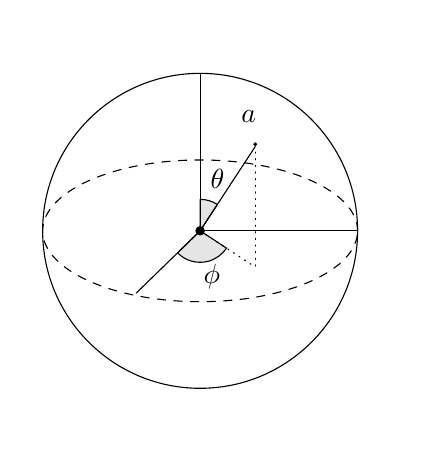
\begin{tikzpicture}
    [line cap=round, line join=round]
    \clip (-2.19,-2.49) rectangle (2.66,2.58);
    \draw [shift={(0,0)}, fill, fill opacity=0.1] (0,0) -- (56.7:0.4) arc (56.7:90.:0.4) -- cycle;
    \draw [shift={(0,0)}, fill, fill opacity=0.1] (0,0) -- (-135.7:0.4) arc (-135.7:-33.2:0.4) -- cycle;
    \draw (0,0) circle (2cm);
    \draw [rotate around={0.:(0.,0.)},dash pattern=on 3pt off 3pt] (0,0) ellipse (2cm and 0.9cm);
    \draw (0,0)-- (0.70,1.07);
    \draw (0,0) -- (0,2);
    \draw (0,0) -- (-0.81,-0.79);
    \draw (0,0) -- (2,0);
    \draw [dotted] (0.7,1) -- (0.7,-0.46);
    \draw [dotted] (0,0) -- (0.7,-0.46);
    \draw (-0.08,-0.3) node[anchor=north west] {$\phi$};
    \draw (0.01,0.9) node[anchor=north west] {$\theta$};
    \draw (0.4,1.65) node[anchor=north west] {$\ket{a}$};
    \scriptsize
    \draw [fill] (0,0) circle (1.5pt);
    \draw [fill] (0.7,1.1) circle (0.5pt);
  \end{tikzpicture}
  \caption{Representación de un ket $\ket{a}\in\mathcal{C}$ en la esfera}
\end{figure}

Pero no podemos realizar esta representación sobre toda la esfera, pues los valores de $\theta$ y $\phi$ no son únicos para cada estado, ya que
\[
  \cos(\theta)\ket{0}+e^{i\phi}\sin(\theta)\ket{1}=-(\cos(\pi-\theta)\ket{0}+e^{i(\pi+\phi)}\sin(\pi-\theta)\ket{1})\,,
\]
solo se diferencian en una fase global. Por lo que los puntos $(\theta,\phi)$ y $(\pi-\theta,\pi+\phi)$ representan el mismo estado físico.

Para evitar esta ambigüedad, se suele restringir el valor de $\theta$ al intervalo $[0, \pi/2)$, lo que corresponde a la mitad superior de la esfera.

Por convenio, se dibuja la esfera sobre los tres ejes espaciales X, Y, Z de tal modo que el ecuador quede en el plano XY, igualmente se considera el eje Z perpendicular a dicho plano.
Los kets de la base canónica computacional se sitúan sobre el eje Z, estando el ket $\ket{0}$ en el eje positivo y el ket $\ket{1}$ sobre el eje negativo.

Esta forma de representación de un estado del cúbit recibe el nombre de \textbf{esfera de Bloch}.

\begin{figure}[H]
  \centering
  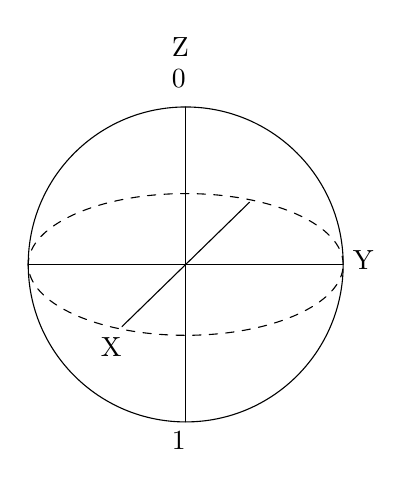
\begin{tikzpicture}
    [line cap=round, line join=round]
    \draw (0,0) circle (2cm);
    \draw [rotate around={0.:(0.,0.)},dash pattern=on 3pt off 3pt] (0,0) ellipse (2cm and 0.9cm);
    \draw (0,0) -- (0,2);
    \draw (0,0) -- (0,-2);
    \draw (0,0) -- (2,0);
    \draw (0,0) -- (-2,0);
    \draw (0,0) -- (-0.81,-0.79);
    \draw (0,0) -- (0.81,0.79);
    \draw (-0.3,3) node[anchor=north west] {Z};
    \draw (-0.3,2.6) node[anchor=north west] {$\ket{0}$};
    \draw (-0.3,-2) node[anchor=north west] {$\ket{1}$};
    \draw (2,0.3) node[anchor=north west] {Y};
    \draw (-1.2,-0.8) node[anchor=north west] {X};
  \end{tikzpicture}
  \caption{Ejes espaciales y representación de la base canónica computacional en la esfera de Bloch}
\end{figure}

\begin{eje}
  El estado $\ket{+} = \frac{1}{\sqrt{2}}(\ket{0} + \ket{1})$ corresponde al punto en el ecuador con $\phi=0$.

  Mientras que $\ket{-} = \frac{1}{\sqrt{2}}(\ket{0} - \ket{1})$ corresponde al punto en el ecuador con $\phi=\pi$.
\end{eje}
